\documentclass{article}
\usepackage{style}

\author{Jorge Gómez Reus}
\date{}
\begin{document}
\maketitle
\tableofcontents
\section{Sistema Lineal}
Es aquel que posee le propiedad de superposición: Si una entrada consiste en la suma ponderada de varias señales, entonces la salida es simplemente la suma ponderada (superposición) de las respuestas del sistema a cada una de las señales.\\
Propiedades: 
\begin{enumerate}
	\item Aditividad:\\
	\begin{figure}[h!]
		\centering
		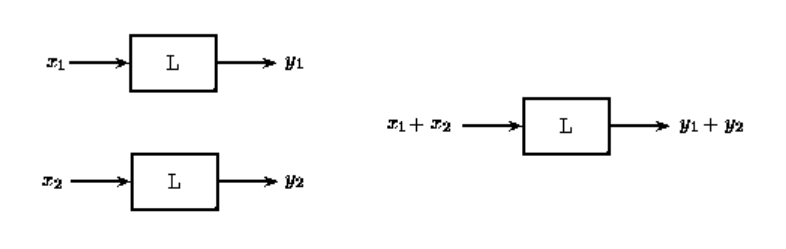
\includegraphics[scale=.8]{img/aditivity}
	\end{figure} 
	\item Escalamiento u Homogeniedad
	\begin{figure}[h!]
		\centering
		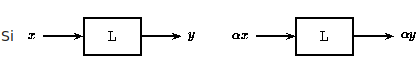
\includegraphics[scale=.8]{img/proportionality}
	\end{figure} 
\end{enumerate}
Las dos propiedades que definen un sistema lineal combinadas se conocen como superposición:
\begin{itemize}
	\item Tiempo continuo: $ax_1(t) + bx_2(t) \rightarrow ay_1(t) + by_2(t)$\\
	$$y[n] = \sum_{k}=a_{k}x_{k}[n] = a_1x_1[n] + a_2x_2[n] + a_3x_3[n] + \ldots$$
	\item Tiempo Discreto: $ax_1[n] + bx_2[n] \rightarrow ay_1[n] + by_2[n]$\\
	$$y[n] = \sum_{k}=a_{k}y_{k}[n] = a_1y_1[n] + a_2y_2[n] + a_3y_3[n] + \ldots$$
\end{itemize}
Una consecuencia directa de la propiedad de superposición es que para sistemas lineales, una entrada que sea cero en todo tiempo da una salida de en todo tiempo.
\section{Ejemplos}
\subsection{Determinar si el sistema es lineal}
\begin{align}
	y(t) = t^2 + tx(t)
\end{align}
Se consideran dos entradas arbitrarias $x_1(t)$ y $x_2(t)$\\
\begin{align}
	x_1(t) \rightarrow y_1(t) = t^2 + tx_1(t)\\
	x_2(t) \rightarrow y_2(t) = t^2 + tx_2(t)
\end{align}

Sea $x_3(t)$ una combinación lineal de $x_1(t)$ y $x_2(t).$ Esto es:\\
\begin{align}
	x_3(t) = ax_1(t) + bx_2(t)
\end{align}
Donde a y b son escalares arbitrarios. Si $x_3(t) $ es la entrada a $S$, entonces la salida correspondiente se expresa como\\
\begin{align}
	y_3(t) &= a(t^2 + tx_1(t)) + b(t^2 + tx_2(t))\\
		   &= at^2 + atx_1(t) + bt^2 + btx_2(t)\\
		   &= (a+b)t^2 + atx_1(t) + btx_2(t)
\end{align}
Se concluye que el sistema no es lineal
\setcounter{equation}{0}
\subsection{Determinar si el sistema es lineal}
\begin{align}
y(t) = x^2(t) + tx(t)
\end{align}
Se consideran dos entradas arbitrarias $x_1(t)$ y $x_2(t)$\\
\begin{align}
x_1(t) \rightarrow y_1(t) = x_1^2(t) + tx_1(t)\\
x_2(t) \rightarrow y_2(t) = x_2^2(t) + tx_2(t)
\end{align}

Sea $x_3(t)$ una combinación lineal de $x_1(t)$ y $x_2(t).$ Esto es:\\
\begin{align}
x_3(t) = ax_1(t) + bx_2(t)
\end{align}
Donde a y b son escalares arbitrarios. Si $x_3(t) $ es la entrada a $S$, entonces la salida correspondiente se expresa como\\
\begin{align}
x_3(t) \rightarrow y_3(t) &= x_3^2(t) + tx_3(t)\\ 
						  &= (ax_1(t) + bx_2(t))^2 + t(ax_1(t) + bx_2(t))\\
						  &= a^2x_1^2(t) + b^2x_2^2(t) + 2abx_1(t)x_2(t) + atx_1(t) + btx_2(t)
\end{align}

y
\begin{align}
y_3(t) &= a_y1(t) + b_y2(t)\\ 
       &= a(x_1^2(t) + tx_1(t)) + b(x_2^2(t) + tx_2(t))\\
       &= ax_1^2(t) + atx_1(t) + bx_2^2(t) + btx_2(t)
\end{align} 
Claramente el sistema no es lineal
\end{document}
